% This must be in the first 5 lines to tell arXiv to use pdfLaTeX, which is strongly recommended.
\pdfoutput=1
% In particular, the hyperref package requires pdfLaTeX in order to break URLs across lines.

\documentclass[11pt]{article}

% Remove the "review" option to generate the final version.
\usepackage[review]{ACL2023}

% Standard package includes
\usepackage{times}
\usepackage{latexsym}

% For proper rendering and hyphenation of words containing Latin characters (including in bib files)
\usepackage[T1]{fontenc}
% For Vietnamese characters
% \usepackage[T5]{fontenc}
% See https://www.latex-project.org/help/documentation/encguide.pdf for other character sets

% This assumes your files are encoded as UTF8
\usepackage[utf8]{inputenc}
\usepackage{float}
% This is not strictly necessary, and may be commented out.
% However, it will improve the layout of the manuscript,
% and will typically save some space.
\usepackage{microtype}

% This is also not strictly necessary, and may be commented out.
% However, it will improve the aesthetics of text in
% the typewriter font.
\usepackage{inconsolata}

\usepackage{graphicx}

% If the title and author information does not fit in the area allocated, uncomment the following
%
%\setlength\titlebox{<dim>}
%
% and set <dim> to something 5cm or larger.

\title{Instructions for ACL 2023 Proceedings}

% Author information can be set in various styles:
% For several authors from the same institution:
% \author{Author 1 \and ... \and Author n \\
%         Address line \\ ... \\ Address line}
% if the names do not fit well on one line use
%         Author 1 \\ {\bf Author 2} \\ ... \\ {\bf Author n} \\
% For authors from different institutions:
% \author{Author 1 \\ Address line \\  ... \\ Address line
%         \And  ... \And
%         Author n \\ Address line \\ ... \\ Address line}
% To start a seperate ``row'' of authors use \AND, as in
% \author{Author 1 \\ Address line \\  ... \\ Address line
%         \AND
%         Author 2 \\ Address line \\ ... \\ Address line \And
%         Author 3 \\ Address line \\ ... \\ Address line}

\author{First Author \\
  Affiliation / Address line 1 \\
  Affiliation / Address line 2 \\
  Affiliation / Address line 3 \\
  \texttt{email@domain} \\\And
  Second Author \\
  Affiliation / Address line 1 \\
  Affiliation / Address line 2 \\
  Affiliation / Address line 3 \\
  \texttt{email@domain} \\}

\begin{document}
\maketitle
\begin{abstract}

\end{abstract}

\section{Introduction}
\section{Methods}

\subsection{Models}
We developed a probing framework for three compact vision--language models:
\textbf{Qwen2-VL-2B}, \textbf{Gemma-3-4B-IT}, and \textbf{FastVLM-0.5}.
All models were used in frozen form, i.e., without updating their parameters,
so that only lightweight probing classifiers were trained on top of their internal
representations. This allows us to isolate the representational capacity of the models
at different layers without confounding effects from fine-tuning.

\subsection{Probing Tasks}
To investigate the distinction between global and local semantic representations,
we designed two probing tasks. The \emph{caption experiment} targets global features
by testing whether the model can align an image with a candidate caption.
For this task, inputs are constructed using the prompt
\texttt{This image contains: \{caption\}. Is this right?},
and the probe performs binary classification of entailment versus non-entailment.
The \emph{category experiment} focuses on local features by probing whether the model
can identify the presence of specific objects. For this task, prompts take the form
\texttt{This image contains the following type of object: \{category\}},
and the probe must predict the correctness of the statement. Both tasks are based
on the MS~COCO dataset, with positive and negative examples sampled to ensure balanced
training and evaluation splits.

\subsection{Representation Extraction}
Our framework computes hidden representations for every transformer layer of a model
given an image--prompt pair. From the token-level hidden states, we derive pooled embeddings
that serve as inputs to the probing classifiers. We implemented a general-purpose
\texttt{pool\_tokens} function that supports multiple pooling strategies, including
CLS token extraction, mean pooling across valid tokens, max pooling, token-index selection,
and a default strategy that retrieves the last non-padding token. Unless otherwise noted,
we employ mean pooling, which aggregates information across the entire input sequence
while respecting attention masks. This yields a single fixed-size vector per input
and per layer, enabling layerwise comparison of representational quality.

\subsection{Probing Classifiers}
On top of the pooled embeddings, we train lightweight classifiers that map the
representations to task labels. For both experiments, we use a simple linear
projection with dropout regularization, optimized with Adam and cross-entropy loss.
The caption experiment is framed as binary classification, while the category experiment
is treated as multi-label prediction with label and mask vectors indicating valid
categories for each image. All probes are trained independently per layer, which allows
us to quantify how well each layer captures global or local semantic information.
Our trainer additionally computes detailed evaluation metrics, including accuracy for
caption entailment and macro-averaged F1, precision, recall, and confusion matrix
statistics for category recognition.

\subsection{Experimental Workflow}
In both experiments, the workflow follows the same high-level structure.
Datasets are preprocessed and split into training and evaluation sets, with
balanced numbers of positive and negative instances. The target model is then
loaded, and representations are computed for all inputs. Probing classifiers are subsequently trained
and evaluated for each layer. After finishing one model, GPU memory is released
and the next model is processed in the same way. The probing results across
layers and models are then aggregated for analysis. This setup ensures that
our experiments are efficient, reproducible, and directly comparable across
models of different architectures and scales.


\section{Results}
To evaluate the performance of the probing classifiers across different layers
and models, we generated a series of plots that visualize key metrics.
For the caption experiment, which focuses on global semantic features, the accuracy per layer
across all three models is shown in Figure~\ref{fig:accuracy_per_layer}. Thus the positive and negative examples are balanced, a random baseline would achieve 50\% accuracy.
\begin{figure}[H]
    \centering
    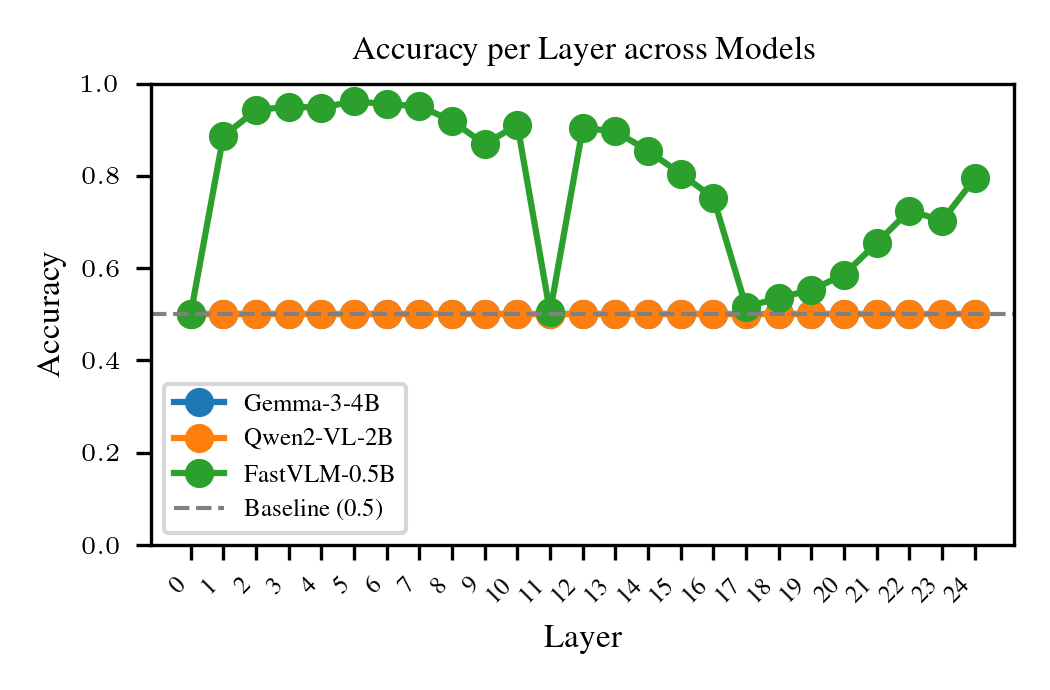
\includegraphics[width=1\linewidth]{figures/global/_combined/accuracy_lines_per_layer.png}
    \caption{Accuracy per layer across all three models.}
    \label{fig:accuracy_per_layer}
\end{figure}

\begin{figure}[H]
    \centering
    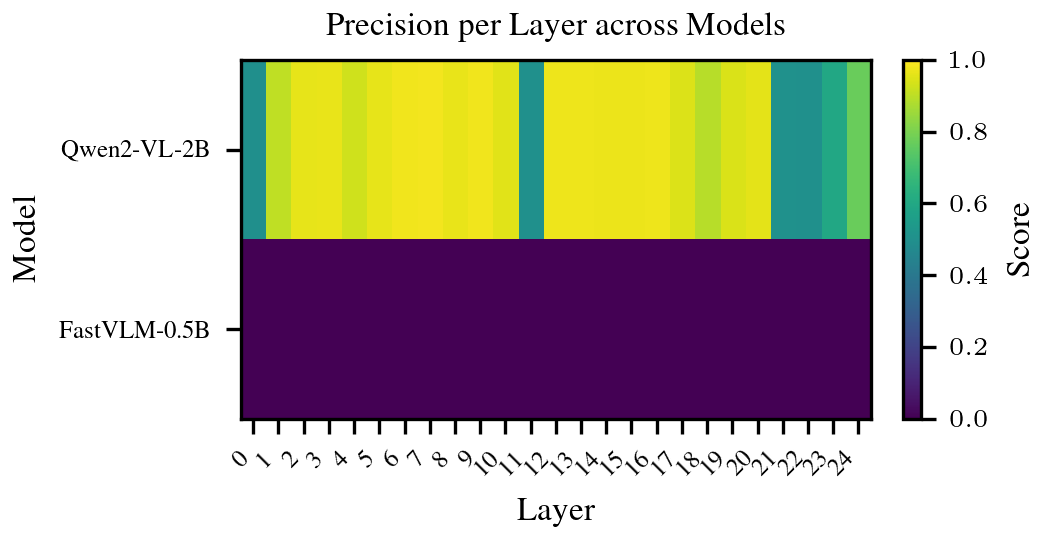
\includegraphics[width=1\linewidth]{figures/global/_combined/precision_heatmap.png}
    \caption{Precision per layer across all three models.}
    \label{fig:precision_per_layer}
\end{figure}

\begin{figure}[H]
    \centering
    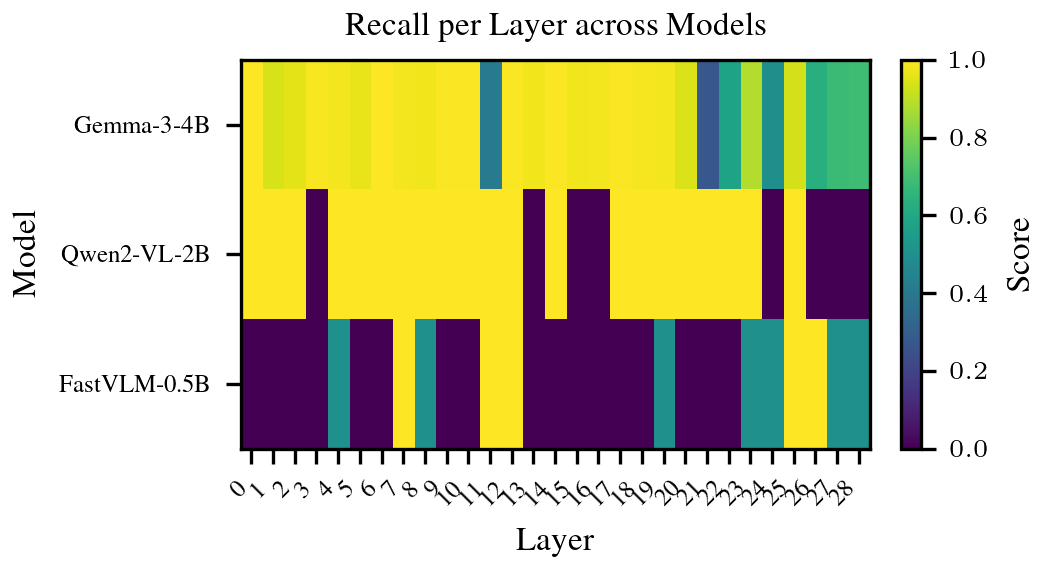
\includegraphics[width=1\linewidth]{figures/global/_combined/recall_heatmap.png}
    \caption{Recall per layer across all three models.}
    \label{fig:recall_per_layer}
\end{figure}






\section{Discussion}
\section{Conclusion}

\section{References}

\nocite{Ando2005,augenstein-etal-2016-stance,andrew2007scalable,rasooli-tetrault-2015,goodman-etal-2016-noise,harper-2014-learning}

The \LaTeX{} and Bib\TeX{} style files provided roughly follow the American Psychological Association format.
If your own bib file is named \texttt{custom.bib}, then placing the following before any appendices in your \LaTeX{} file will generate the references section for you:
\begin{quote}
\begin{verbatim}
\bibliographystyle{acl_natbib}
\bibliography{custom}
\end{verbatim}
\end{quote}
You can obtain the complete ACL Anthology as a Bib\TeX{} file from \url{https://aclweb.org/anthology/anthology.bib.gz}.
To include both the Anthology and your own .bib file, use the following instead of the above.
\begin{quote}
\begin{verbatim}
\bibliographystyle{acl_natbib}
\bibliography{custom}
\end{verbatim}
\end{quote}
Please see Section~\ref{sec:bibtex} for information on preparing Bib\TeX{} files.

\subsection{Appendices}

Use \verb|\appendix| before any appendix section to switch the section numbering over to letters. See Appendix~\ref{sec:appendix} for an example.


\bibliography{anthology,custom}
\bibliographystyle{acl_natbib}

\appendix

\section{Example Appendix}

\end{document}
